% Options for packages loaded elsewhere
\PassOptionsToPackage{unicode}{hyperref}
\PassOptionsToPackage{hyphens}{url}
%
\documentclass[
  ignorenonframetext,
]{beamer}
\usepackage{pgfpages}
\setbeamertemplate{caption}[numbered]
\setbeamertemplate{caption label separator}{: }
\setbeamercolor{caption name}{fg=normal text.fg}
\beamertemplatenavigationsymbolsempty
% Prevent slide breaks in the middle of a paragraph
\widowpenalties 1 10000
\raggedbottom
\setbeamertemplate{part page}{
  \centering
  \begin{beamercolorbox}[sep=16pt,center]{part title}
    \usebeamerfont{part title}\insertpart\par
  \end{beamercolorbox}
}
\setbeamertemplate{section page}{
  \centering
  \begin{beamercolorbox}[sep=12pt,center]{part title}
    \usebeamerfont{section title}\insertsection\par
  \end{beamercolorbox}
}
\setbeamertemplate{subsection page}{
  \centering
  \begin{beamercolorbox}[sep=8pt,center]{part title}
    \usebeamerfont{subsection title}\insertsubsection\par
  \end{beamercolorbox}
}
\AtBeginPart{
  \frame{\partpage}
}
\AtBeginSection{
  \ifbibliography
  \else
    \frame{\sectionpage}
  \fi
}
\AtBeginSubsection{
  \frame{\subsectionpage}
}
\usepackage{lmodern}
\usepackage{amssymb,amsmath}
\usepackage{ifxetex,ifluatex}
\ifnum 0\ifxetex 1\fi\ifluatex 1\fi=0 % if pdftex
  \usepackage[T1]{fontenc}
  \usepackage[utf8]{inputenc}
  \usepackage{textcomp} % provide euro and other symbols
\else % if luatex or xetex
  \usepackage{unicode-math}
  \defaultfontfeatures{Scale=MatchLowercase}
  \defaultfontfeatures[\rmfamily]{Ligatures=TeX,Scale=1}
\fi
% Use upquote if available, for straight quotes in verbatim environments
\IfFileExists{upquote.sty}{\usepackage{upquote}}{}
\IfFileExists{microtype.sty}{% use microtype if available
  \usepackage[]{microtype}
  \UseMicrotypeSet[protrusion]{basicmath} % disable protrusion for tt fonts
}{}
\makeatletter
\@ifundefined{KOMAClassName}{% if non-KOMA class
  \IfFileExists{parskip.sty}{%
    \usepackage{parskip}
  }{% else
    \setlength{\parindent}{0pt}
    \setlength{\parskip}{6pt plus 2pt minus 1pt}}
}{% if KOMA class
  \KOMAoptions{parskip=half}}
\makeatother
\usepackage{xcolor}
\IfFileExists{xurl.sty}{\usepackage{xurl}}{} % add URL line breaks if available
\IfFileExists{bookmark.sty}{\usepackage{bookmark}}{\usepackage{hyperref}}
\hypersetup{
  pdftitle={Multivariate Statistics with R},
  pdfauthor={Aja Murray, Aja.Murray@ed.ac.uk},
  hidelinks,
  pdfcreator={LaTeX via pandoc}}
\urlstyle{same} % disable monospaced font for URLs
\newif\ifbibliography
\usepackage{color}
\usepackage{fancyvrb}
\newcommand{\VerbBar}{|}
\newcommand{\VERB}{\Verb[commandchars=\\\{\}]}
\DefineVerbatimEnvironment{Highlighting}{Verbatim}{commandchars=\\\{\}}
% Add ',fontsize=\small' for more characters per line
\usepackage{framed}
\definecolor{shadecolor}{RGB}{248,248,248}
\newenvironment{Shaded}{\begin{snugshade}}{\end{snugshade}}
\newcommand{\AlertTok}[1]{\textcolor[rgb]{0.94,0.16,0.16}{#1}}
\newcommand{\AnnotationTok}[1]{\textcolor[rgb]{0.56,0.35,0.01}{\textbf{\textit{#1}}}}
\newcommand{\AttributeTok}[1]{\textcolor[rgb]{0.77,0.63,0.00}{#1}}
\newcommand{\BaseNTok}[1]{\textcolor[rgb]{0.00,0.00,0.81}{#1}}
\newcommand{\BuiltInTok}[1]{#1}
\newcommand{\CharTok}[1]{\textcolor[rgb]{0.31,0.60,0.02}{#1}}
\newcommand{\CommentTok}[1]{\textcolor[rgb]{0.56,0.35,0.01}{\textit{#1}}}
\newcommand{\CommentVarTok}[1]{\textcolor[rgb]{0.56,0.35,0.01}{\textbf{\textit{#1}}}}
\newcommand{\ConstantTok}[1]{\textcolor[rgb]{0.00,0.00,0.00}{#1}}
\newcommand{\ControlFlowTok}[1]{\textcolor[rgb]{0.13,0.29,0.53}{\textbf{#1}}}
\newcommand{\DataTypeTok}[1]{\textcolor[rgb]{0.13,0.29,0.53}{#1}}
\newcommand{\DecValTok}[1]{\textcolor[rgb]{0.00,0.00,0.81}{#1}}
\newcommand{\DocumentationTok}[1]{\textcolor[rgb]{0.56,0.35,0.01}{\textbf{\textit{#1}}}}
\newcommand{\ErrorTok}[1]{\textcolor[rgb]{0.64,0.00,0.00}{\textbf{#1}}}
\newcommand{\ExtensionTok}[1]{#1}
\newcommand{\FloatTok}[1]{\textcolor[rgb]{0.00,0.00,0.81}{#1}}
\newcommand{\FunctionTok}[1]{\textcolor[rgb]{0.00,0.00,0.00}{#1}}
\newcommand{\ImportTok}[1]{#1}
\newcommand{\InformationTok}[1]{\textcolor[rgb]{0.56,0.35,0.01}{\textbf{\textit{#1}}}}
\newcommand{\KeywordTok}[1]{\textcolor[rgb]{0.13,0.29,0.53}{\textbf{#1}}}
\newcommand{\NormalTok}[1]{#1}
\newcommand{\OperatorTok}[1]{\textcolor[rgb]{0.81,0.36,0.00}{\textbf{#1}}}
\newcommand{\OtherTok}[1]{\textcolor[rgb]{0.56,0.35,0.01}{#1}}
\newcommand{\PreprocessorTok}[1]{\textcolor[rgb]{0.56,0.35,0.01}{\textit{#1}}}
\newcommand{\RegionMarkerTok}[1]{#1}
\newcommand{\SpecialCharTok}[1]{\textcolor[rgb]{0.00,0.00,0.00}{#1}}
\newcommand{\SpecialStringTok}[1]{\textcolor[rgb]{0.31,0.60,0.02}{#1}}
\newcommand{\StringTok}[1]{\textcolor[rgb]{0.31,0.60,0.02}{#1}}
\newcommand{\VariableTok}[1]{\textcolor[rgb]{0.00,0.00,0.00}{#1}}
\newcommand{\VerbatimStringTok}[1]{\textcolor[rgb]{0.31,0.60,0.02}{#1}}
\newcommand{\WarningTok}[1]{\textcolor[rgb]{0.56,0.35,0.01}{\textbf{\textit{#1}}}}
\usepackage{graphicx,grffile}
\makeatletter
\def\maxwidth{\ifdim\Gin@nat@width>\linewidth\linewidth\else\Gin@nat@width\fi}
\def\maxheight{\ifdim\Gin@nat@height>\textheight\textheight\else\Gin@nat@height\fi}
\makeatother
% Scale images if necessary, so that they will not overflow the page
% margins by default, and it is still possible to overwrite the defaults
% using explicit options in \includegraphics[width, height, ...]{}
\setkeys{Gin}{width=\maxwidth,height=\maxheight,keepaspectratio}
% Set default figure placement to htbp
\makeatletter
\def\fps@figure{htbp}
\makeatother
\setlength{\emergencystretch}{3em} % prevent overfull lines
\providecommand{\tightlist}{%
  \setlength{\itemsep}{0pt}\setlength{\parskip}{0pt}}
\setcounter{secnumdepth}{-\maxdimen} % remove section numbering

\title{Multivariate Statistics with R}
\subtitle{Principal Components Analysis}
\author{Aja Murray,
\href{mailto:Aja.Murray@ed.ac.uk}{\nolinkurl{Aja.Murray@ed.ac.uk}}}
\date{}

\begin{document}
\frame{\titlepage}

\begin{frame}{Overview}
\protect\hypertarget{overview}{}

\begin{itemize}
\tightlist
\item
  Week 1: Dimension Reduction (PCA and EFA)
\item
  Week 2: SEM I - Confirmatory Factor Analysis
\item
  Week 3: SEM II - Path Analysis
\item
  Week 4: SEM III - Full SEM
\item
  Week 5: SEM IV - Practical Issues in SEM
\end{itemize}

\end{frame}

\begin{frame}{This Week}
\protect\hypertarget{this-week}{}

\begin{itemize}
\tightlist
\item
  Techniques

  \begin{itemize}
  \tightlist
  \item
    Principal Components Analysis (PCA)
  \item
    Exploratory Factor Analysis (EFA)
  \end{itemize}
\item
  Key Functions

  \begin{itemize}
  \tightlist
  \item
    vss( )
  \item
    fa.parallel( )
  \item
    principal( )
  \item
    fa( )
  \end{itemize}
\item
  Reading: \emph{Principal Components Analysis} and \emph{Exploratory
  Factor Analysis} Chapters (on \emph{Learn} under `Reading')
\end{itemize}

\end{frame}

\begin{frame}{Learning Outcomes}
\protect\hypertarget{learning-outcomes}{}


\includegraphics{D:/Teaching and Supervision/Psychology/MVwR_1920/Draft Lectures/learning outcomes.jpg}

\begin{itemize}
\tightlist
\item
  Understand the principles of dimension reduction
\item
  Understand thd difference between PCA and EFA
\item
  Know how to perform and interpret PCA and EFA in R
\end{itemize}

\end{frame}

\begin{frame}{Dimension Reduction}
\protect\hypertarget{dimension-reduction}{}

\begin{itemize}
\tightlist
\item
  Summarise a set of variables in terms of a smaller number of
  dimensions

  \begin{itemize}
  \tightlist
  \item
    e.g., can 10 aggression items summarised in terms of `physical' and
    `verbal' aggression dimensions?
  \end{itemize}

  \begin{enumerate}
  \tightlist
  \item
    I hit someone
  \item
    I kicked someone
  \item
    I shoved someone
  \item
    I battered someone
  \item
    I physically hurt someone on purpose
  \item
    I deliberately insulted someone
  \item
    I swore at someone
  \item
    I threatened to hurt someone
  \item
    I called someone a nasty name to their face
  \item
    I shouted mean things at someone
  \end{enumerate}
\end{itemize}

\end{frame}

\begin{frame}{Uses of dimension reduction techniques}
\protect\hypertarget{uses-of-dimension-reduction-techniques}{}

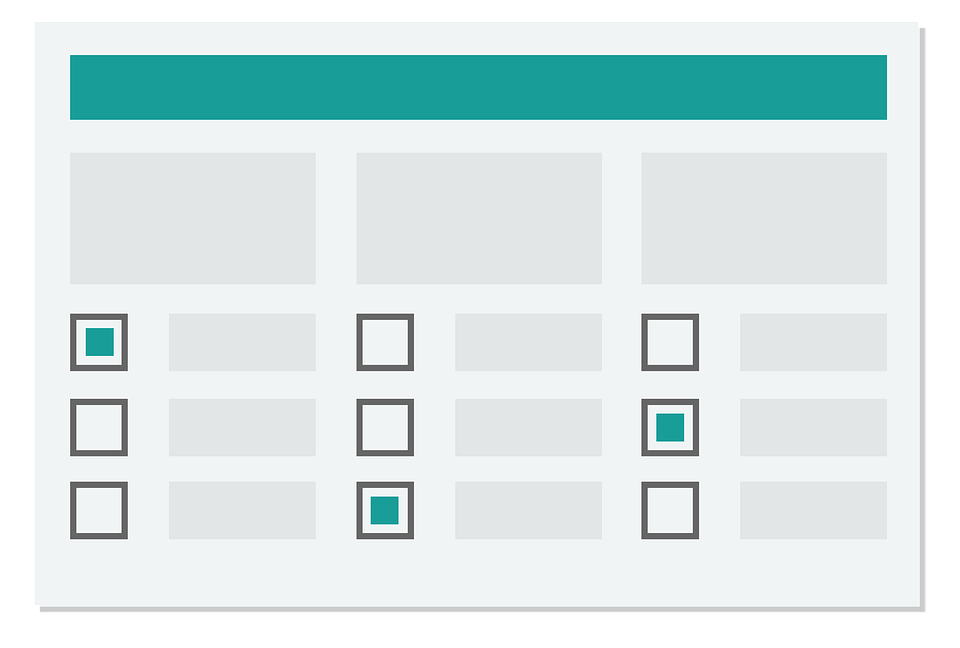
\includegraphics[width=0.3\textwidth,height=\textheight]{D:/Teaching and Supervision/Psychology/MVwR_1920/Draft Lectures/Questionnaire.png}

\begin{itemize}
\tightlist
\item
  Theory testing

  \begin{itemize}
  \tightlist
  \item
    What are the number and nature of dimensions that best describe a
    theoretical construct?
  \end{itemize}
\item
  Test construction

  \begin{itemize}
  \tightlist
  \item
    How should I group my items into subscales?
  \item
    Which items are the best measures of my constructs?
  \end{itemize}
\item
  Pragmatic

  \begin{itemize}
  \tightlist
  \item
    I have multicollinearity issues/too many variables, how can I
    defensibly combine my variables?
  \end{itemize}
\end{itemize}

\end{frame}

\begin{frame}[fragile]{Our running example}
\protect\hypertarget{our-running-example}{}

\begin{itemize}
\tightlist
\item
  A researcher has collected n=1000 responses to our 10 aggression items
\item
  We'll use this data to illustrate dimension reduction techniques
\end{itemize}

\begin{Shaded}
\begin{Highlighting}[]
\KeywordTok{library}\NormalTok{(psych)}
\KeywordTok{describe}\NormalTok{(agg.items)}
\end{Highlighting}
\end{Shaded}

\begin{verbatim}
##        vars    n mean   sd median trimmed  mad   min  max range  skew kurtosis
## item1     1 1000 0.04 0.99   0.06    0.05 0.95 -3.06 3.25  6.32 -0.07     0.17
## item2     2 1000 0.02 0.98   0.00    0.02 0.96 -2.94 3.34  6.28  0.04     0.06
## item3     3 1000 0.03 0.99   0.04    0.03 1.05 -3.00 3.72  6.73  0.02    -0.15
## item4     4 1000 0.03 1.00   0.05    0.04 0.99 -3.47 3.47  6.93 -0.15     0.26
## item5     5 1000 0.01 0.98  -0.02    0.00 0.93 -3.20 3.05  6.25 -0.02     0.24
## item6     6 1000 0.02 0.97   0.02    0.02 0.97 -3.15 2.99  6.14 -0.01    -0.03
## item7     7 1000 0.06 1.03   0.10    0.07 1.03 -2.98 3.20  6.18 -0.10    -0.17
## item8     8 1000 0.02 1.05   0.03    0.03 1.07 -3.16 3.00  6.15 -0.06    -0.16
## item9     9 1000 0.00 1.01   0.01    0.00 1.04 -2.93 3.30  6.23  0.00     0.03
## item10   10 1000 0.03 1.01   0.02    0.03 1.02 -2.66 3.40  6.06  0.08     0.06
##          se
## item1  0.03
## item2  0.03
## item3  0.03
## item4  0.03
## item5  0.03
## item6  0.03
## item7  0.03
## item8  0.03
## item9  0.03
## item10 0.03
\end{verbatim}

\end{frame}

\begin{frame}[fragile]{PCA}
\protect\hypertarget{pca}{}

\begin{itemize}
\tightlist
\item
  Starts with a correlation matrix
\end{itemize}

\begin{Shaded}
\begin{Highlighting}[]
\CommentTok{#compute the correlation matrix for the aggression items}
\KeywordTok{round}\NormalTok{(}\KeywordTok{cor}\NormalTok{(agg.items),}\DecValTok{2}\NormalTok{)}
\end{Highlighting}
\end{Shaded}

\begin{verbatim}
##        item1 item2 item3 item4 item5 item6 item7 item8 item9 item10
## item1   1.00  0.55  0.50  0.46  0.59  0.14  0.22  0.17  0.17   0.15
## item2   0.55  1.00  0.55  0.53  0.66  0.10  0.16  0.14  0.11   0.09
## item3   0.50  0.55  1.00  0.45  0.59  0.11  0.17  0.15  0.13   0.10
## item4   0.46  0.53  0.45  1.00  0.52  0.17  0.22  0.21  0.18   0.14
## item5   0.59  0.66  0.59  0.52  1.00  0.09  0.12  0.09  0.12   0.05
## item6   0.14  0.10  0.11  0.17  0.09  1.00  0.57  0.59  0.43   0.46
## item7   0.22  0.16  0.17  0.22  0.12  0.57  1.00  0.83  0.65   0.64
## item8   0.17  0.14  0.15  0.21  0.09  0.59  0.83  1.00  0.64   0.65
## item9   0.17  0.11  0.13  0.18  0.12  0.43  0.65  0.64  1.00   0.50
## item10  0.15  0.09  0.10  0.14  0.05  0.46  0.64  0.65  0.50   1.00
\end{verbatim}

\end{frame}

\begin{frame}{What PCA does}
\protect\hypertarget{what-pca-does}{}

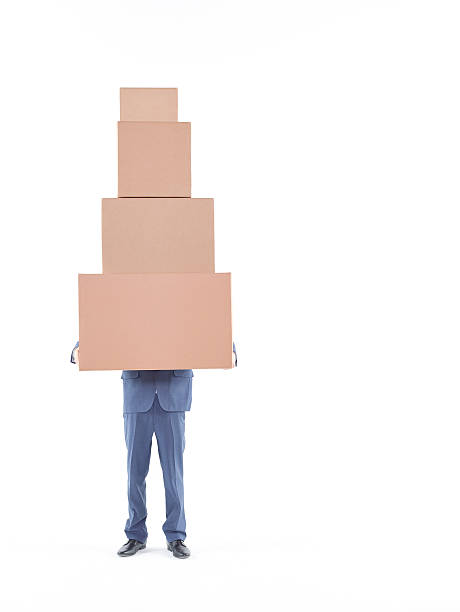
\includegraphics[width=0.2\textwidth,height=\textheight]{D:/Teaching and Supervision/Psychology/MVwR_1920/Draft Lectures/packages.jpg}

\begin{itemize}
\tightlist
\item
  Repackages the variance from the correlation matrix into a set of
  \textbf{components}
\item
  Components = orthogonal (i.e.,uncorrelated) linear combinations of the
  original variables

  \begin{itemize}
  \tightlist
  \item
    1st component is the linear combination that accounts for the most
    possible variance
  \item
    2nd accounts for second-largest after the variance accounted for by
    the first is removed
  \item
    3rd\ldots etc\ldots{}
  \end{itemize}
\item
  Each component accounts for as much remaining variance as possible
\item
  There are as many components are there were variables in original
  correlation matrix
\end{itemize}

\end{frame}

\begin{frame}{Eigendecomposition}
\protect\hypertarget{eigendecomposition}{}

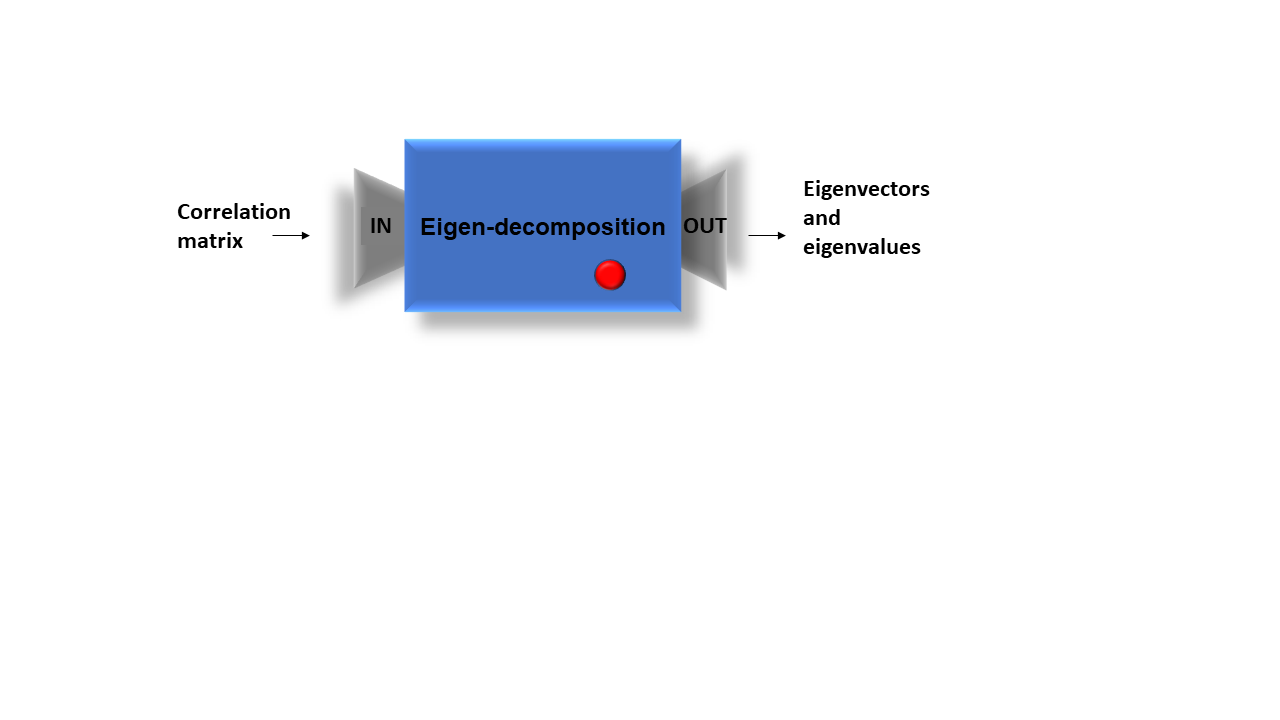
\includegraphics[width=0.7\textwidth,height=\textheight]{D:/Teaching and Supervision/Psychology/MVwR_1920/Draft Lectures/eigendecomposition.png}

\begin{itemize}
\tightlist
\item
  Components are formed using an \textbf{eigen-decomposition} of the
  correlation matrix
\item
  Eigen-decomposition is a transformation of the correlation matrix to
  re-express it in terms of \textbf{eigenvalues} and
  \textbf{eigenvectors}
\end{itemize}

\end{frame}

\begin{frame}[fragile]{Eigenvalues and eigenvectors}
\protect\hypertarget{eigenvalues-and-eigenvectors}{}

\begin{verbatim}
## [1] "e1" "e2" "e3" "e4" "e5"
\end{verbatim}

\begin{verbatim}
##       component1 component2 component3 component4 component5
## item1 "w11"      "w12"      "w13"      "w14"      "w15"     
## item2 "w21"      "w22"      "w23"      "w24"      "w25"     
## item3 "w31"      "w32"      "w33"      "w34"      "w35"     
## item4 "w41"      "w42"      "w43"      "w44"      "w45"     
## item5 "w51"      "w52"      "w53"      "w54"      "w55"
\end{verbatim}

\begin{itemize}
\tightlist
\item
  There is one eigenvector and one eigenvalue for each component
\item
  Eigenvalues are a measure of the size of the variance packaged into a
  component

  \begin{itemize}
  \tightlist
  \item
    Larger eigenvalues mean that the component accounts for a large
    proportion of the variance in the original correlation matrix
  \end{itemize}
\item
  Eigenvectors are sets of \textbf{weights} (one weight per variable in
  original correlation matrix)

  \begin{itemize}
  \tightlist
  \item
    e.g., if we had 5 variables each eigenvector would contain 5 weights
  \item
    Larger weights mean a variable makes a bigger contribution to the
    component
  \end{itemize}
\end{itemize}

\end{frame}

\begin{frame}[fragile]{Eigen-decomposition of aggression item
correlation matrix}
\protect\hypertarget{eigen-decomposition-of-aggression-item-correlation-matrix}{}

\begin{itemize}
\tightlist
\item
  We can use the eigen() function to conduct an eigen-decomposition for
  our 10 aggression items
\end{itemize}

\begin{Shaded}
\begin{Highlighting}[]
\KeywordTok{eigen}\NormalTok{(}\KeywordTok{cor}\NormalTok{(agg.items))}
\end{Highlighting}
\end{Shaded}

\begin{verbatim}
## eigen() decomposition
## $values
##  [1] 3.9977423 2.5837392 0.5858985 0.5671836 0.5009288 0.4965831 0.4225958
##  [8] 0.3607065 0.3128699 0.1717523
## 
## $vectors
##            [,1]       [,2]        [,3]        [,4]        [,5]         [,6]
##  [1,] 0.2980678 -0.3105964  0.19851746 -0.24903189  0.57168243 -0.417393473
##  [2,] 0.2882799 -0.3777720 -0.03399598 -0.01076730  0.05472171  0.055514376
##  [3,] 0.2779476 -0.3353941  0.13168206 -0.36757017 -0.60221848  0.351807641
##  [4,] 0.2925436 -0.2769057 -0.34042730  0.76092346  0.07010032  0.201518615
##  [5,] 0.2818286 -0.4020106  0.02001509 -0.07849765 -0.04712347 -0.125201727
##  [6,] 0.3020308  0.2530536 -0.77725918 -0.33745416 -0.05867762 -0.221980727
##  [7,] 0.3847791  0.2979569  0.08445852  0.02018479 -0.03179630 -0.001215889
##  [8,] 0.3751978  0.3182154  0.02172432  0.04108306 -0.03809047  0.060524708
##  [9,] 0.3271809  0.2617339  0.40779147  0.29425946 -0.34581474 -0.479133989
## [10,] 0.3141465  0.2957357  0.21856960 -0.12261233  0.41819873  0.600114540
##              [,7]        [,8]        [,9]       [,10]
##  [1,] -0.42876137  0.13456206  0.08797477  0.05038315
##  [2,]  0.67631712  0.33043594  0.44694048 -0.02205635
##  [3,] -0.39181652  0.05387290  0.12194310  0.00892539
##  [4,] -0.30726127 -0.04002698  0.02959575 -0.02085343
##  [5,]  0.32215853 -0.48221596 -0.63081507  0.01598419
##  [6,] -0.02890193 -0.20193357  0.17844694 -0.02366001
##  [7,]  0.01125821  0.39228584 -0.32712107 -0.70255996
##  [8,]  0.05057443  0.39249094 -0.30502683  0.70784423
##  [9,]  0.03262345 -0.32316417  0.34096961  0.02546861
## [10,]  0.04958755 -0.42722232  0.17515082 -0.01904281
\end{verbatim}

\end{frame}

\begin{frame}{BREAK 1}
\protect\hypertarget{break-1}{}

\begin{itemize}
\tightlist
\item
  Time for a pause
\item
  Quiz question:

  \begin{itemize}
  \tightlist
  \item
    What is the name of the process by which a correlation matrix is
    transformed into eigenvectors and eigenvalues?

    \begin{itemize}
    \item
      \begin{enumerate}
      [A)]
      \tightlist
      \item
        eigen-sedimentation
      \end{enumerate}
    \item
      \begin{enumerate}
      [A)]
      \setcounter{enumi}{1}
      \tightlist
      \item
        eigen-consolidation
      \end{enumerate}
    \item
      \begin{enumerate}
      [A)]
      \setcounter{enumi}{2}
      \tightlist
      \item
        eigen-diversification
      \end{enumerate}
    \item
      \begin{enumerate}
      [A)]
      \setcounter{enumi}{3}
      \tightlist
      \item
        eigen-decomposition
      \end{enumerate}
    \end{itemize}
  \end{itemize}
\end{itemize}

\end{frame}

\begin{frame}{WELCOME BACK 1}
\protect\hypertarget{welcome-back-1}{}

\begin{itemize}
\item
  Welcome back!
\item
  The answer to the quiz question is\ldots{}

  \begin{itemize}
  \item
    \begin{enumerate}
    [A)]
    \tightlist
    \item
      eigen-sedimentation
    \end{enumerate}
  \item
    \begin{enumerate}
    [A)]
    \setcounter{enumi}{1}
    \tightlist
    \item
      eigen-consolidation
    \end{enumerate}
  \item
    \begin{enumerate}
    [A)]
    \setcounter{enumi}{2}
    \tightlist
    \item
      eigen-diversification
    \end{enumerate}
  \item
    \begin{enumerate}
    [A)]
    \setcounter{enumi}{3}
    \tightlist
    \item
      \textbf{eigen-decomposition}
    \end{enumerate}
  \end{itemize}
\end{itemize}

\end{frame}

\begin{frame}{How many components to keep?}
\protect\hypertarget{how-many-components-to-keep}{}

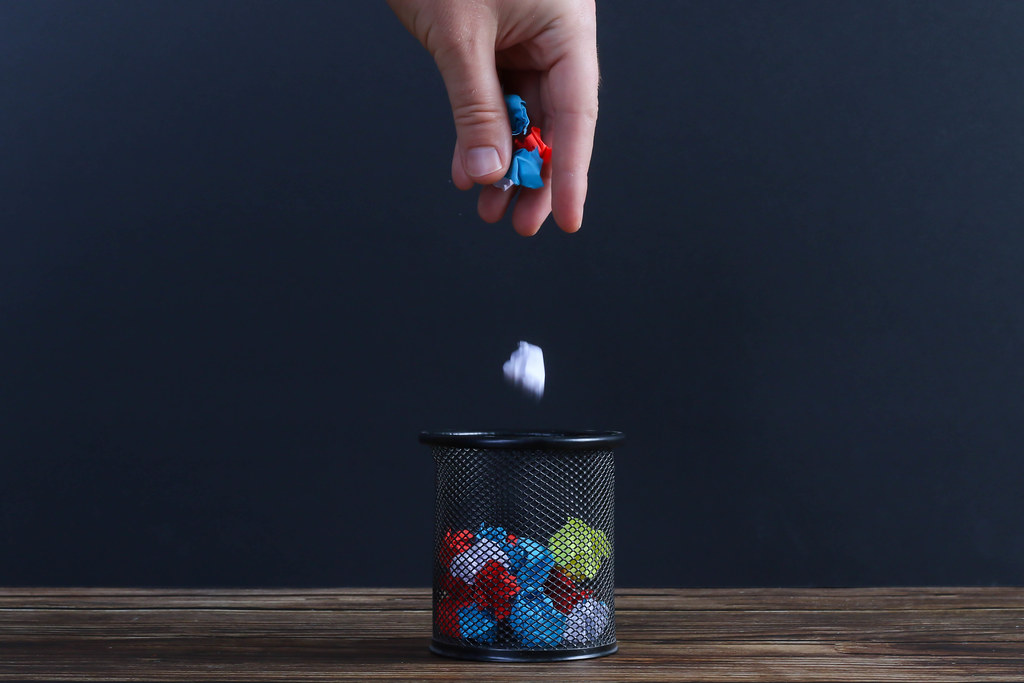
\includegraphics[width=0.3\textwidth,height=\textheight]{D:/Teaching and Supervision/Psychology/MVwR_1920/Draft Lectures/Wastepaper.jpg}

\begin{itemize}
\tightlist
\item
  Eigen-decomposition repackages the variance but does not reduce our
  dimensions
\item
  Dimension reduction comes from keeping only the largest components
\item
  Assume the others can be dropped with little loss of information
\item
  Our decisions on how many components to keep can be guided by several
  methods

  \begin{itemize}
  \tightlist
  \item
    Scree plot
  \item
    Minimum average partial test (MAP)
  \item
    Parallel analysis
  \end{itemize}
\end{itemize}

\end{frame}

\begin{frame}{Other considerations in how many components to keep}
\protect\hypertarget{other-considerations-in-how-many-components-to-keep}{}

\includegraphics[width=0.3\textwidth,height=\textheight]{D:/Teaching and Supervision/Psychology/MVwR_1920/Draft Lectures/Magnify.jpg}

\begin{itemize}
\tightlist
\item
  Substantive considerations

  \begin{itemize}
  \tightlist
  \item
    Do the selected components make theoretical sense?
  \end{itemize}
\item
  Practical considerations

  \begin{itemize}
  \tightlist
  \item
    Are some components too `minor' to be reliable?
  \end{itemize}
\end{itemize}

\end{frame}

\begin{frame}{Kaiser criterion}
\protect\hypertarget{kaiser-criterion}{}


\includegraphics[width=0.3\textwidth,height=\textheight]{D:/Teaching and Supervision/Psychology/MVwR_1920/Draft Lectures/do not.png}

\begin{itemize}
\tightlist
\item
  Keeps number of components with eigenvalue \textgreater1
\item
  DO NOT USE Kaiser criterion
\item
  Often suggests keeping far too many components
\end{itemize}

\end{frame}

\begin{frame}{Scree plot}
\protect\hypertarget{scree-plot}{}

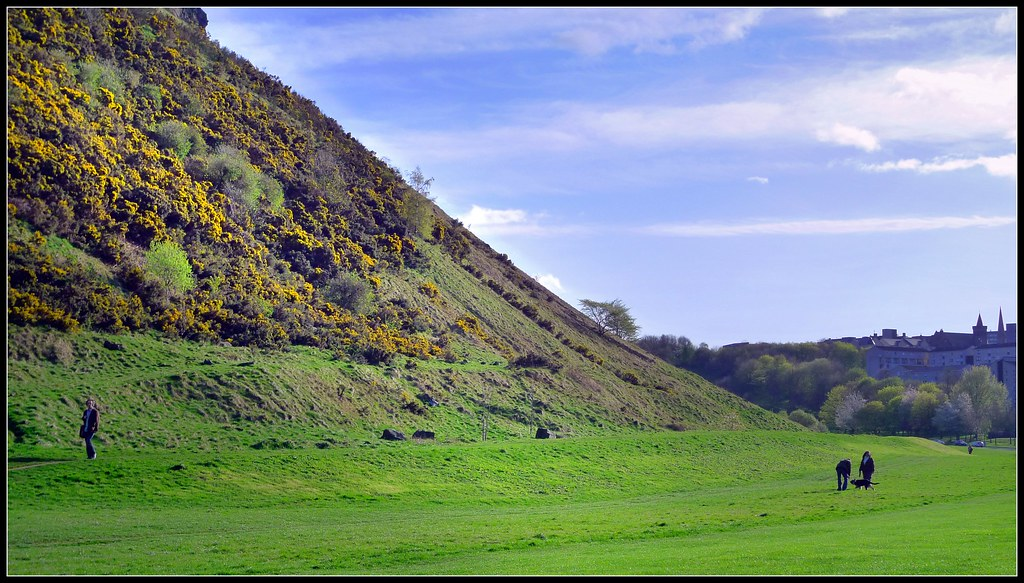
\includegraphics[width=0.3\textwidth,height=\textheight]{D:/Teaching and Supervision/Psychology/MVwR_1920/Draft Lectures/scree_salisbury.jpg}

\begin{itemize}
\tightlist
\item
  Based on plotting the eigenvalues
\item
  Looking for a sudden change of slope
\item
  Assumed to potentially reflect point at which components become
  substantively unimportant
\end{itemize}

\end{frame}

\begin{frame}{Constructing a scree plot}
\protect\hypertarget{constructing-a-scree-plot}{}

\includegraphics{Week-7---PCA_files/figure-beamer/Scree plot example-1.pdf}

\begin{itemize}
\tightlist
\item
  Eigenvalue plot

  \begin{itemize}
  \tightlist
  \item
    x-axis is component number
  \item
    y-axis is eigenvalue for each component
  \end{itemize}
\item
  Keep the components with eigenvalues above a kink in the plot
\end{itemize}

\end{frame}

\begin{frame}[fragile]{Further scree plot examples}
\protect\hypertarget{further-scree-plot-examples}{}

\begin{itemize}
\tightlist
\item
  Scree plots vary in how easy it is to interpret them
\end{itemize}

\begin{verbatim}
## [1] 10
\end{verbatim}

\includegraphics{Week-7---PCA_files/figure-beamer/Scree plot example 1-1.pdf}

\end{frame}

\begin{frame}[fragile]{Further scree plot examples}
\protect\hypertarget{further-scree-plot-examples-1}{}

\begin{verbatim}
## [1] 10
\end{verbatim}

\includegraphics{Week-7---PCA_files/figure-beamer/Scree plot example 2-1.pdf}

\end{frame}

\begin{frame}[fragile]{Further scree plot examples}
\protect\hypertarget{further-scree-plot-examples-2}{}

\begin{verbatim}
## [1] 10
\end{verbatim}

\includegraphics{Week-7---PCA_files/figure-beamer/Scree plot example 3-1.pdf}

\end{frame}

\begin{frame}{Minimum average partial test (MAP)}
\protect\hypertarget{minimum-average-partial-test-map}{}

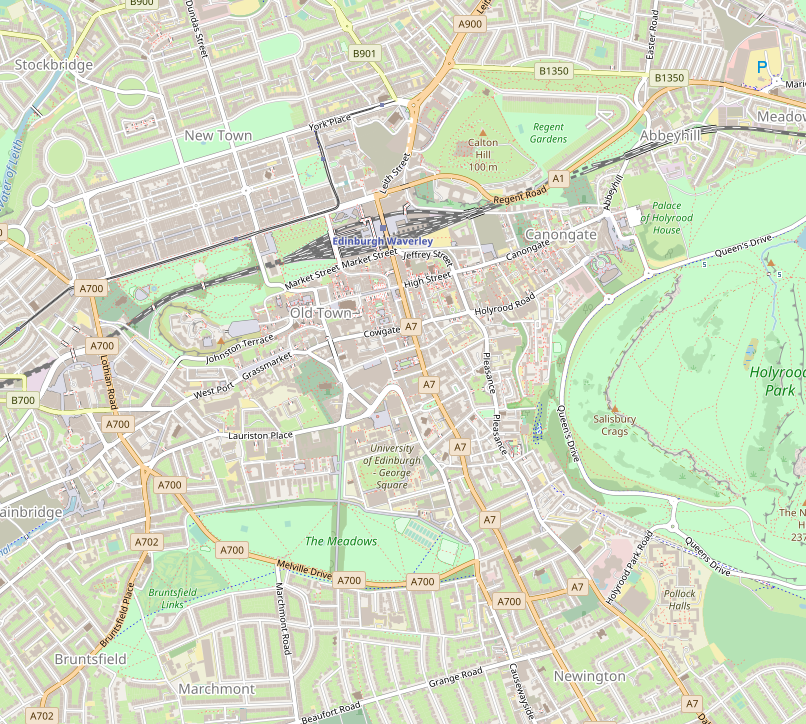
\includegraphics[width=0.4\textwidth,height=\textheight]{D:/Teaching and Supervision/Psychology/MVwR_1920/Draft Lectures/map_edinburgh.png}

\begin{itemize}
\tightlist
\item
  Extracts components iteratively from the correlation matrix
\item
  Computes the average squared partial correlation after each extraction
\item
  At first this quantity goes down with each component extracted but
  then it starts to increase again
\item
  MAP keeps the components from point at which the average squared
  partial correlation is at its smallest
\end{itemize}

\end{frame}

\begin{frame}[fragile]{MAP test for the aggression items}
\protect\hypertarget{map-test-for-the-aggression-items}{}

\begin{itemize}
\tightlist
\item
  We can obtain the results of the MAP test via the vss( ) function from
  the psych package
\end{itemize}

\begin{Shaded}
\begin{Highlighting}[]
\KeywordTok{library}\NormalTok{(psych)}
\KeywordTok{vss}\NormalTok{(agg.items)}
\end{Highlighting}
\end{Shaded}

\includegraphics{Week-7---PCA_files/figure-beamer/MAP test for aggression-1.pdf}

\begin{verbatim}
## 
## Very Simple Structure
## Call: vss(x = agg.items)
## Although the VSS complexity 1 shows  7  factors, it is probably more reasonable to think about  3  factors
## VSS complexity 2 achieves a maximimum of 0.92  with  2  factors
## 
## The Velicer MAP achieves a minimum of 0.03  with  2  factors 
## BIC achieves a minimum of  NA  with  2  factors
## Sample Size adjusted BIC achieves a minimum of  NA  with  2  factors
## 
## Statistics by number of factors 
##   vss1 vss2   map dof   chisq prob sqresid  fit RMSEA  BIC SABIC complex
## 1 0.64 0.00 0.149  35 2.4e+03 0.00     8.7 0.64  0.26 2166  2277     1.0
## 2 0.87 0.92 0.030  26 2.0e+01 0.77     2.0 0.92  0.00 -159   -77     1.0
## 3 0.87 0.92 0.058  18 9.8e+00 0.94     1.9 0.92  0.00 -115   -57     1.1
## 4 0.77 0.91 0.098  11 3.5e+00 0.98     1.7 0.93  0.00  -72   -38     1.2
## 5 0.71 0.91 0.155   5 1.6e+00 0.90     1.3 0.95  0.00  -33   -17     1.2
## 6 0.70 0.92 0.247   0 4.1e-02   NA     1.2 0.95    NA   NA    NA     1.3
## 7 0.87 0.91 0.354  -4 5.2e-07   NA     1.6 0.93    NA   NA    NA     1.2
## 8 0.87 0.91 0.665  -7 1.2e-09   NA     1.7 0.93    NA   NA    NA     1.2
##    eChisq    SRMR  eCRMS eBIC
## 1 4.2e+03 2.2e-01 0.2438 3920
## 2 6.3e+00 8.3e-03 0.0110 -173
## 3 3.3e+00 6.1e-03 0.0096 -121
## 4 1.2e+00 3.6e-03 0.0074  -75
## 5 4.7e-01 2.3e-03 0.0068  -34
## 6 9.0e-03 3.2e-04     NA   NA
## 7 1.1e-07 1.1e-06     NA   NA
## 8 3.7e-10 6.4e-08     NA   NA
\end{verbatim}

\end{frame}

\begin{frame}[fragile]{The MAP values}
\protect\hypertarget{the-map-values}{}

\begin{itemize}
\tightlist
\item
  The averaged squared partial correlation values
\end{itemize}

\begin{Shaded}
\begin{Highlighting}[]
\NormalTok{VSS}\OperatorTok{$}\NormalTok{map}
\end{Highlighting}
\end{Shaded}

\begin{verbatim}
## [1] 0.14943600 0.02968596 0.05792221 0.09808270 0.15494014 0.24701416 0.35436970
## [8] 0.66486374
\end{verbatim}

\end{frame}

\begin{frame}{Parallel analysis}
\protect\hypertarget{parallel-analysis}{}

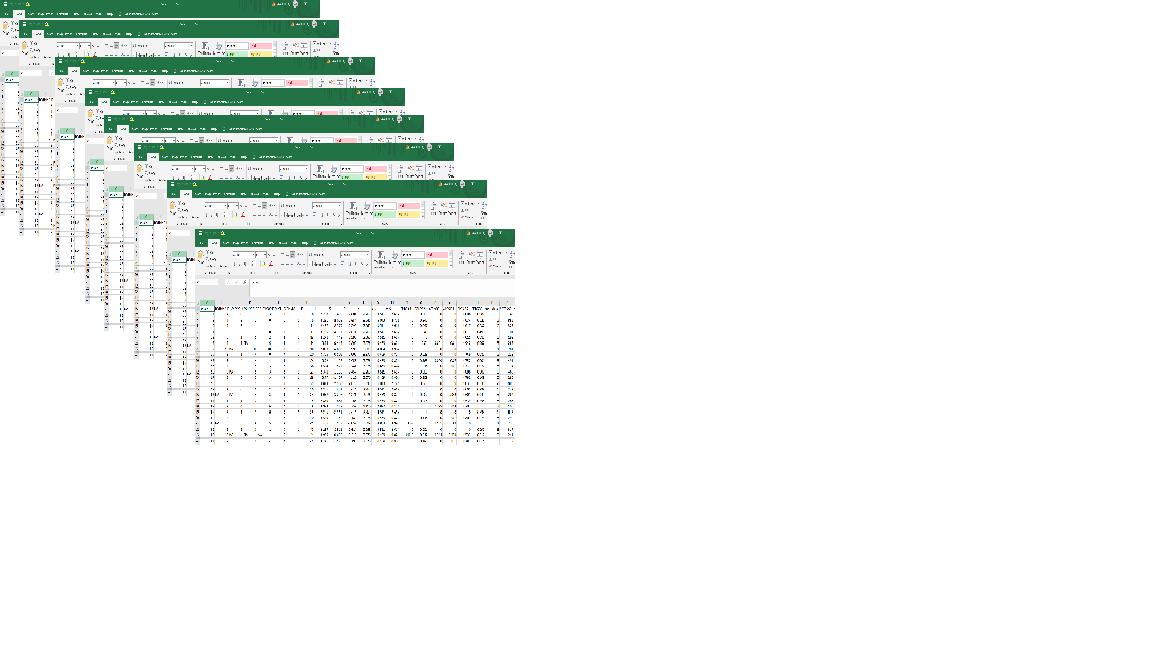
\includegraphics[width=0.4\textwidth,height=\textheight]{D:/Teaching and Supervision/Psychology/MVwR_1920/Draft Lectures/simulated_datasets.png}

\begin{itemize}
\tightlist
\item
  Simulates datasets with same number of participants and variables but
  no correlations
\item
  Computes an eigen-decomposition for the simulated datasets
\item
  Compares the average eigenvalue across the simulated datasets for each
  component
\item
  If a real eigenvalue exceeds the corresponding average eigenvalue from
  the simulated datasets it is retained
\item
  We can also use alternative methods to compare our real versus
  simulated eigenvalues

  \begin{itemize}
  \tightlist
  \item
    e.g.~95\% percentile of the simulated eigenvalue distributions
  \end{itemize}
\end{itemize}

\end{frame}

\begin{frame}[fragile]{Parallel analysis for the aggression items}
\protect\hypertarget{parallel-analysis-for-the-aggression-items}{}

\begin{Shaded}
\begin{Highlighting}[]
\KeywordTok{fa.parallel}\NormalTok{(agg.items, }\DataTypeTok{n.iter=}\DecValTok{500}\NormalTok{)}
\end{Highlighting}
\end{Shaded}

\includegraphics{Week-7---PCA_files/figure-beamer/parallel analysis-1.pdf}

\begin{verbatim}
## Parallel analysis suggests that the number of factors =  2  and the number of components =  2
\end{verbatim}

\end{frame}

\begin{frame}[fragile]{The fa.parallel( ) function}
\protect\hypertarget{the-fa.parallel-function}{}

\begin{itemize}
\tightlist
\item
  Notice the function also gives us a scree plot
\item
  We can use this to find a point of inflection

  \begin{itemize}
  \tightlist
  \item
    Use the `PC Actual Data' datapoints
  \end{itemize}
\item
  However, if we want to include a scree plot in a report we should
  construct our own, e.g.:
\end{itemize}

\begin{Shaded}
\begin{Highlighting}[]
\NormalTok{eigenvalues<-}\KeywordTok{eigen}\NormalTok{(}\KeywordTok{cor}\NormalTok{(agg.items))}\OperatorTok{$}\NormalTok{values}
\KeywordTok{plot}\NormalTok{(eigenvalues, }\DataTypeTok{type =} \StringTok{'b'}\NormalTok{, }\DataTypeTok{pch =} \DecValTok{16}\NormalTok{, }
     \DataTypeTok{main =} \StringTok{"Scree Plot"}\NormalTok{, }\DataTypeTok{xlab=}\StringTok{""}\NormalTok{, }\DataTypeTok{ylab=}\StringTok{"Eigenvalues"}\NormalTok{)}
\KeywordTok{axis}\NormalTok{(}\DecValTok{1}\NormalTok{, }\DataTypeTok{at =} \DecValTok{1}\OperatorTok{:}\DecValTok{10}\NormalTok{, }\DataTypeTok{labels =} \DecValTok{1}\OperatorTok{:}\DecValTok{10}\NormalTok{)}
\end{Highlighting}
\end{Shaded}

\includegraphics{Week-7---PCA_files/figure-beamer/code for a scree plot-1.pdf}

\end{frame}

\begin{frame}{Limitations of scree, MAP, and parallel analysis}
\protect\hypertarget{limitations-of-scree-map-and-parallel-analysis}{}

\begin{itemize}
\tightlist
\item
  There is no one right answer about the number of components to retain
\item
  Scree plot, MAP and parallel analysis frequently disagree
\item
  Each method has weaknesses

  \begin{itemize}
  \tightlist
  \item
    Scree plots are subjective and may have multiple or no obvious kinks
  \item
    Parallel analysis sometimes suggest too many components
  \item
    MAP sometimes suggests too few components
  \end{itemize}
\item
  Examining the PCA solutions should also form part of the decision
\end{itemize}

\end{frame}

\begin{frame}{BREAK 2}
\protect\hypertarget{break-2}{}

\begin{itemize}
\tightlist
\item
  Time for a pause
\item
  Quiz question:

  \begin{itemize}
  \tightlist
  \item
    Which components are retained based on a scree plot?

    \begin{itemize}
    \item
      \begin{enumerate}
      [A)]
      \tightlist
      \item
        Those with eigenvalues up to and including the kink
      \end{enumerate}
    \item
      \begin{enumerate}
      [A)]
      \setcounter{enumi}{1}
      \tightlist
      \item
        Those with eigenvalues \textgreater2
      \end{enumerate}
    \item
      \begin{enumerate}
      [A)]
      \setcounter{enumi}{2}
      \tightlist
      \item
        Those with eigenvalues before the kink
      \end{enumerate}
    \item
      \begin{enumerate}
      [A)]
      \setcounter{enumi}{3}
      \tightlist
      \item
        Those up to the point where the average squared partial
        correlation is at its minimum
      \end{enumerate}
    \end{itemize}
  \end{itemize}
\end{itemize}

\end{frame}

\begin{frame}{WELCOME BACK 2}
\protect\hypertarget{welcome-back-2}{}

\begin{itemize}
\tightlist
\item
  Welcome back!
\item
  The answer to the quiz question is\ldots{}

  \begin{itemize}
  \tightlist
  \item
    Which components are retained based on a scree plot?

    \begin{itemize}
    \item
      \begin{enumerate}
      [A)]
      \tightlist
      \item
        Those with eigenvalues up to and including the kink
      \end{enumerate}
    \item
      \begin{enumerate}
      [A)]
      \setcounter{enumi}{1}
      \tightlist
      \item
        Those with eigenvalues \textgreater2
      \end{enumerate}
    \item
      \begin{enumerate}
      [A)]
      \setcounter{enumi}{2}
      \tightlist
      \item
        \textbf{Those with eigenvalues before the kink}
      \end{enumerate}
    \item
      \begin{enumerate}
      [A)]
      \setcounter{enumi}{3}
      \tightlist
      \item
        Those up to the point where the average squared partial
        correlation is at its minimum
      \end{enumerate}
    \end{itemize}
  \end{itemize}
\end{itemize}

\end{frame}

\begin{frame}[fragile]{Running a PCA with a reduced number of
components}
\protect\hypertarget{running-a-pca-with-a-reduced-number-of-components}{}

\begin{itemize}
\tightlist
\item
  We can run a PCA keeping just a selected number of components
\item
  We do this using the principal() function from then psych package
\item
  We supply the dataframe or correlation matrix as the first argument
\item
  We specify the number of components to retain with the nfactors=
  argument
\item
  It can be useful to compare and constrast the solutions with different
  numbers of components

  \begin{itemize}
  \tightlist
  \item
    Allows us to check which solutions make most sense based on
    substantive/practical considerations
  \end{itemize}
\end{itemize}

\begin{Shaded}
\begin{Highlighting}[]
\NormalTok{PC2<-}\KeywordTok{principal}\NormalTok{(agg.items, }\DataTypeTok{nfactors=}\DecValTok{2}\NormalTok{) }
\NormalTok{PC3<-}\KeywordTok{principal}\NormalTok{(agg.items, }\DataTypeTok{nfactors=}\DecValTok{3}\NormalTok{) }
\end{Highlighting}
\end{Shaded}

\end{frame}

\begin{frame}{Interpreting the components}
\protect\hypertarget{interpreting-the-components}{}

\begin{itemize}
\tightlist
\item
  Once we have decided how many components to keep (or to help us
  decide) we examine the PCA solution
\item
  We do this based on the component loadings

  \begin{itemize}
  \tightlist
  \item
    Component loadings are calculated from the values in the
    eigenvectors
  \item
    They can be interpreted as the correlations between variables and
    components
  \end{itemize}
\end{itemize}

\end{frame}

\begin{frame}[fragile]{The component loadings}
\protect\hypertarget{the-component-loadings}{}

\begin{itemize}
\tightlist
\item
  Component loading matrix
\item
  RC1 and RC2 columns show the component loadings
\end{itemize}

\begin{Shaded}
\begin{Highlighting}[]
\NormalTok{PC2<-}\KeywordTok{principal}\NormalTok{(}\DataTypeTok{r=}\NormalTok{agg.items, }\DataTypeTok{nfactors=}\DecValTok{2}\NormalTok{)}
\NormalTok{PC2}\OperatorTok{$}\NormalTok{loadings}
\end{Highlighting}
\end{Shaded}

\begin{verbatim}
## 
## Loadings:
##        RC1   RC2  
## item1  0.125 0.767
## item2        0.836
## item3        0.771
## item4  0.152 0.719
## item5        0.857
## item6  0.723      
## item7  0.895 0.140
## item8  0.902 0.103
## item9  0.770 0.109
## item10 0.786      
## 
##                  RC1   RC2
## SS loadings    3.395 3.187
## Proportion Var 0.339 0.319
## Cumulative Var 0.339 0.658
\end{verbatim}

\end{frame}

\begin{frame}{Interpreting the components}
\protect\hypertarget{interpreting-the-components-1}{}

\begin{enumerate}
\tightlist
\item
  I hit someone
\item
  I kicked someone
\item
  I shoved someone
\item
  I battered someone
\item
  I physically hurt someone on purpose
\item
  I deliberately insulted someone
\item
  I swore at someone
\item
  I threatened to hurt someone
\item
  I called someone a nasty name to their face
\item
  I shouted mean things at someone
\end{enumerate}

\end{frame}

\begin{frame}{Rotation of components}
\protect\hypertarget{rotation-of-components}{}

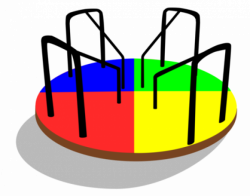
\includegraphics{D:/Teaching and Supervision/Psychology/MVwR_1920/Draft Lectures/rotation.png}

\begin{itemize}
\tightlist
\item
  Rotation takes an initial PCA solution and transforms it to make it
  more interpretable
\item
  An initial PCA solution typically has:

  \begin{itemize}
  \tightlist
  \item
    has high loadings on the first component
  \item
    has a mix of positive and negative loadings on subsequent components
  \item
    is difficult to interpret
  \end{itemize}
\item
  We typically try to achieve \emph{simple structure} with a rotation

  \begin{itemize}
  \tightlist
  \item
    each item has a high loading on one component and close to zero
    loading on all others
  \end{itemize}
\end{itemize}

\end{frame}

\begin{frame}[fragile]{Initial PCA solution for the aggression items}
\protect\hypertarget{initial-pca-solution-for-the-aggression-items}{}

\begin{Shaded}
\begin{Highlighting}[]
\NormalTok{PC_initial<-}\KeywordTok{principal}\NormalTok{(}\DataTypeTok{r=}\NormalTok{agg.items, }\DataTypeTok{nfactors=}\DecValTok{2}\NormalTok{, }\DataTypeTok{rotate=}\StringTok{'none'}\NormalTok{)}
\NormalTok{PC_initial}\OperatorTok{$}\NormalTok{loadings}
\end{Highlighting}
\end{Shaded}

\begin{verbatim}
## 
## Loadings:
##        PC1    PC2   
## item1   0.596  0.499
## item2   0.576  0.607
## item3   0.556  0.539
## item4   0.585  0.445
## item5   0.563  0.646
## item6   0.604 -0.407
## item7   0.769 -0.479
## item8   0.750 -0.511
## item9   0.654 -0.421
## item10  0.628 -0.475
## 
##                  PC1   PC2
## SS loadings    3.998 2.584
## Proportion Var 0.400 0.258
## Cumulative Var 0.400 0.658
\end{verbatim}

\end{frame}

\begin{frame}{Different types of rotation}
\protect\hypertarget{different-types-of-rotation}{}

\begin{itemize}
\tightlist
\item
  The initial (unrotated) loading matrix is transformed by
  multiplication by a \emph{transformation matrix}
\item
  Different transformation matrices are used to achieve different
  transformations
\item
  The most important distinction is between \emph{orthogonal} versus
  \emph{oblique} rotations

  \begin{itemize}
  \tightlist
  \item
    Orthogonal rotations force the components to remain uncorrelated

    \begin{itemize}
    \tightlist
    \item
      They include varimax, quartimax and equamax
    \end{itemize}
  \item
    Oblique rotations allow the components to be correlated

    \begin{itemize}
    \tightlist
    \item
      They include oblimin, promax, direct oblimin, and quartimin
    \end{itemize}
  \end{itemize}
\end{itemize}

\end{frame}

\begin{frame}{Choosing a rotation}
\protect\hypertarget{choosing-a-rotation}{}

\begin{itemize}
\tightlist
\item
  Orthogonal rotations are useful for e.g.~reducing multicollinearity in
  regression
\item
  Oblique rotations better reflect the reality that psychological
  constructs tend to be correlated
\item
  Advice: use an oblique rotation and switch to orthogonal if
  correlation is very low

  \begin{itemize}
  \tightlist
  \item
    Oblimin is a good choice for oblique rotation
  \item
    Varimax is a good choice for orthogonal rotation
  \item
    \ldots{} but trying a few and comparing is a good idea
  \end{itemize}
\end{itemize}

\end{frame}

\begin{frame}{Interpreting an oblique rotation}
\protect\hypertarget{interpreting-an-oblique-rotation}{}

\begin{itemize}
\tightlist
\item
  When an orthogonal rotation is used only one loading matrix is
  produced
\item
  When an oblique rotation is used two loading matrices are produced:

  \begin{itemize}
  \tightlist
  \item
    \emph{structure matrix} (correlations between the components and the
    variables)
  \item
    \emph{pattern matrix} (regression weights from the components to the
    variables)
  \end{itemize}
\item
  Pattern is likely to be most useful for interpreting the components
\end{itemize}

\end{frame}

\begin{frame}[fragile]{PCA solution for the aggression items using an
oblique rotation}
\protect\hypertarget{pca-solution-for-the-aggression-items-using-an-oblique-rotation}{}

\begin{Shaded}
\begin{Highlighting}[]
\NormalTok{PC2<-}\KeywordTok{principal}\NormalTok{(}\DataTypeTok{r=}\NormalTok{agg.items, }\DataTypeTok{nfactors=}\DecValTok{2}\NormalTok{, }\DataTypeTok{rotate=}\StringTok{'oblimin'}\NormalTok{)}
\end{Highlighting}
\end{Shaded}

\begin{verbatim}
## Loading required namespace: GPArotation
\end{verbatim}

\begin{Shaded}
\begin{Highlighting}[]
\NormalTok{PC2}\OperatorTok{$}\NormalTok{loadings}
\end{Highlighting}
\end{Shaded}

\begin{verbatim}
## 
## Loadings:
##        TC1    TC2   
## item1          0.762
## item2          0.843
## item3          0.773
## item4          0.710
## item5          0.868
## item6   0.728       
## item7   0.899       
## item8   0.909       
## item9   0.774       
## item10  0.796       
## 
##                  TC1   TC2
## SS loadings    3.417 3.151
## Proportion Var 0.342 0.315
## Cumulative Var 0.342 0.657
\end{verbatim}

\end{frame}

\begin{frame}[fragile]{PCA solution for the aggression items using an
oblique rotation}
\protect\hypertarget{pca-solution-for-the-aggression-items-using-an-oblique-rotation-1}{}

\begin{Shaded}
\begin{Highlighting}[]
\NormalTok{PC2<-}\KeywordTok{principal}\NormalTok{(}\DataTypeTok{r=}\NormalTok{agg.items, }\DataTypeTok{nfactors=}\DecValTok{2}\NormalTok{, }\DataTypeTok{rotate=}\StringTok{'oblimin'}\NormalTok{)}
\NormalTok{PC2}\OperatorTok{$}\NormalTok{Phi}
\end{Highlighting}
\end{Shaded}

\begin{verbatim}
##           TC1       TC2
## TC1 1.0000000 0.2012285
## TC2 0.2012285 1.0000000
\end{verbatim}

\end{frame}

\begin{frame}{BREAK 3}
\protect\hypertarget{break-3}{}

\begin{itemize}
\tightlist
\item
  Time for a pause
\item
  Quiz question:

  \begin{itemize}
  \tightlist
  \item
    Under an oblique rotation which matrix contains the weights for the
    regression of the components on the original variables?

    \begin{itemize}
    \item
      \begin{enumerate}
      [A)]
      \tightlist
      \item
        pattern matrix
      \end{enumerate}
    \item
      \begin{enumerate}
      [A)]
      \setcounter{enumi}{1}
      \tightlist
      \item
        structure matrix
      \end{enumerate}
    \item
      \begin{enumerate}
      [a)]
      \setcounter{enumi}{2}
      \tightlist
      \item
        eigenvector matrix
      \end{enumerate}
    \item
      \begin{enumerate}
      [A)]
      \setcounter{enumi}{3}
      \tightlist
      \item
        eigenvalue matrix
      \end{enumerate}
    \end{itemize}
  \end{itemize}
\end{itemize}

\end{frame}

\begin{frame}{WELCOME BACK 3}
\protect\hypertarget{welcome-back-3}{}

\begin{itemize}
\tightlist
\item
  Welcome back!
\item
  The answer to the quiz question is..

  \begin{itemize}
  \item
    Under an oblique rotation which matrix contains the weights for the
    regression of the components on the original variables?
  \item
    \begin{enumerate}
    [A)]
    \tightlist
    \item
      \textbf{pattern matrix}
    \end{enumerate}
  \item
    \begin{enumerate}
    [A)]
    \setcounter{enumi}{1}
    \tightlist
    \item
      structure matrix
    \end{enumerate}
  \item
    \begin{enumerate}
    [a)]
    \setcounter{enumi}{2}
    \tightlist
    \item
      eigenvector matrix
    \end{enumerate}
  \item
    \begin{enumerate}
    [A)]
    \setcounter{enumi}{3}
    \tightlist
    \item
      eigenvalue matrix
    \end{enumerate}
  \end{itemize}
\end{itemize}

\end{frame}

\begin{frame}[fragile]{How good is my PCA solution?}
\protect\hypertarget{how-good-is-my-pca-solution}{}

\begin{itemize}
\tightlist
\item
  A good PCA solution explains the variance of the original correlation
  matrix in as few components as possible
\end{itemize}

\begin{Shaded}
\begin{Highlighting}[]
\KeywordTok{principal}\NormalTok{(}\DataTypeTok{r=}\NormalTok{agg.items, }\DataTypeTok{nfactors=}\DecValTok{2}\NormalTok{, }\DataTypeTok{rotate=}\StringTok{'oblimin'}\NormalTok{)}
\end{Highlighting}
\end{Shaded}

\begin{verbatim}
## Principal Components Analysis
## Call: principal(r = agg.items, nfactors = 2, rotate = "oblimin")
## Standardized loadings (pattern matrix) based upon correlation matrix
##          TC1   TC2   h2   u2 com
## item1   0.06  0.76 0.60 0.40   1
## item2  -0.03  0.84 0.70 0.30   1
## item3   0.01  0.77 0.60 0.40   1
## item4   0.09  0.71 0.54 0.46   1
## item5  -0.07  0.87 0.74 0.26   1
## item6   0.73  0.00 0.53 0.47   1
## item7   0.90  0.03 0.82 0.18   1
## item8   0.91 -0.01 0.82 0.18   1
## item9   0.77  0.02 0.60 0.40   1
## item10  0.80 -0.05 0.62 0.38   1
## 
##                        TC1  TC2
## SS loadings           3.42 3.16
## Proportion Var        0.34 0.32
## Cumulative Var        0.34 0.66
## Proportion Explained  0.52 0.48
## Cumulative Proportion 0.52 1.00
## 
##  With component correlations of 
##     TC1 TC2
## TC1 1.0 0.2
## TC2 0.2 1.0
## 
## Mean item complexity =  1
## Test of the hypothesis that 2 components are sufficient.
## 
## The root mean square of the residuals (RMSR) is  0.06 
##  with the empirical chi square  327.09  with prob <  7.8e-54 
## 
## Fit based upon off diagonal values = 0.98
\end{verbatim}

\end{frame}

\begin{frame}{Computing scores for the components}
\protect\hypertarget{computing-scores-for-the-components}{}

\begin{itemize}
\tightlist
\item
  After conducting a PCA you may want to create scores for the new
  dimensions

  \begin{itemize}
  \tightlist
  \item
    e.g., to use in a regression
  \end{itemize}
\item
  Simplest method is to sum the scores for all items with loadings
  \textgreater\textbar.3\textbar{}
\item
  Better method is to compute them taking into account the weights
\end{itemize}

\end{frame}

\begin{frame}[fragile]{Computing component scores in R}
\protect\hypertarget{computing-component-scores-in-r}{}

\begin{Shaded}
\begin{Highlighting}[]
\NormalTok{PC<-}\KeywordTok{principal}\NormalTok{(}\DataTypeTok{r=}\NormalTok{agg.items, }\DataTypeTok{nfactors=}\DecValTok{2}\NormalTok{, }\DataTypeTok{rotate=}\StringTok{'oblimin'}\NormalTok{)}
\NormalTok{scores<-PC}\OperatorTok{$}\NormalTok{scores}
\KeywordTok{head}\NormalTok{(scores)}
\end{Highlighting}
\end{Shaded}

\begin{verbatim}
##             TC1         TC2
## [1,] -0.8076707 -0.24798919
## [2,]  0.3926649  0.04542934
## [3,] -1.7003994 -0.21919339
## [4,]  0.5818213  0.40088290
## [5,]  0.2749693 -0.65484794
## [6,] -0.2999026  1.79142578
\end{verbatim}

\end{frame}

\begin{frame}{Reporting a PCA}
\protect\hypertarget{reporting-a-pca}{}

\begin{itemize}
\tightlist
\item
  Main principles: transparency and reproducibility
\item
  Method

  \begin{itemize}
  \tightlist
  \item
    Methods used to decide on number of factors
  \item
    Rotation method
  \end{itemize}
\item
  Results

  \begin{itemize}
  \tightlist
  \item
    Results of MAP, parallel analysis, scree test (\& any other
    considerations in choice of number of components)
  \item
    How many components were retained
  \item
    The loading matrix for the chosen solution (pattern for oblique
    rotations)
  \item
    Correlations between components (for oblique rotations)
  \item
    Variance expained by components
  \item
    Labelling and interpretation of the components
  \end{itemize}
\end{itemize}

\end{frame}

\begin{frame}{PCA Summary}
\protect\hypertarget{pca-summary}{}

\begin{itemize}
\tightlist
\item
  PCA is a common dimension reduction technique
\item
  Steps are:

  \begin{itemize}
  \tightlist
  \item
    Decide how many components to keep (scree plot, parallel analysis,
    MAP test)
  \item
    Rotate (orthogonal versus oblique)
  \item
    Interpret solution (loadings, component correlations, variance
    explained)
  \end{itemize}
\item
  There are many subjective decision points - critical thinking is
  needed
\item
  Number of components is arguably most important decision
\end{itemize}

\end{frame}

\begin{frame}{END OF PCA}
\protect\hypertarget{end-of-pca}{}


\includegraphics{D:/Teaching and Supervision/Psychology/MVwR_1920/Draft Lectures/celebration_emoji.jpg}

\begin{itemize}
\tightlist
\item
  End of PCA section!
\item
  Next we will cover \textbf{exploratory factor analysis}
\end{itemize}

\end{frame}

\end{document}
